\documentclass[11pt]{article}

\usepackage[a4paper,margin=1in]{geometry}
\usepackage[T1]{fontenc}
\usepackage[utf8]{inputenc}
\usepackage{lmodern}
\usepackage{amsmath,amssymb,amsthm,mathtools}
\usepackage{graphicx}
\usepackage{booktabs}
\usepackage{microtype}
\usepackage[numbers,sort&compress]{natbib}
\usepackage[colorlinks=true,linkcolor=blue,citecolor=blue,urlcolor=blue]{hyperref}

\graphicspath{{./}}

\newcommand{\Tr}{\operatorname{Tr}}
\newcommand{\supp}{\operatorname{supp}}

\title{Cross-Scale Locality Signal in Echo-Based Hardware Benchmarks from q14 to q80}
\author{Lenna}
\date{March 21, 2026}

\begin{document}

\maketitle

\begin{abstract}
We report a staged hardware evidence snapshot across q14, q20, q24, q32, and q80 echo-based scrambling benchmarks, with emphasis on locality-sensitive overlap-versus-far-disjoint controls. The strongest large-system evidence remains subset-proxy: for q20, q24, q32, and q80, shallow-depth readout-mitigated subset contrasts remain large and positive, showing a clear signal above a pure-noise baseline under fixed control geometry. At q14, the strongest admissible checkpoint-level hardware anchor remains the corrected local-fold zero-noise-extrapolated overlap-minus-disjoint separation at depth 2, selected from a broader mixed q14 hardware-control picture. At q80, the subset evidence reported here is still a first \texttt{S\_A = 0..9} pilot only, while an exploratory full-register bonus analysis based on a mirrored block-$Z$ fallback observable yields a smaller but still structured residual locality signal. We interpret these results as strong staged continuity for locality-sensitive echo observables across scale, while keeping explicit the gap between the current echo-family observables, subset-level diagnostics, and the still-unresolved fixed-observable operator Loschmidt echo target.
\end{abstract}

\section{Introduction}

Information scrambling is central to current discussions of quantum chaos, nonequilibrium many-body dynamics, and black-hole information flow
\cite{hayden2007blackholes,sekino2008fast,maldacena2016bound}.
Operationally, the problem is to determine whether initially local information remains geometrically identifiable under time evolution, or whether it disperses into highly nonlocal operator structure.
The resulting diagnostics include out-of-time-ordered correlators (OTOCs), Loschmidt echoes, and related recovery or overlap experiments
\cite{yan2020information,vermersch2019probing,mi2021scrambling}.

The present project does not start from an abstract OTOC protocol in isolation.
Instead, it starts from an existing hardware-tested echo workflow built around the quantity called \texttt{perturbed\_echo} in the repository, and asks whether the same hardware control logic already exhibits a locality-sensitive signal robust enough to support a careful bridge toward operator Loschmidt echo (OLE).
That bridge must be staged rather than semantic.
The repository's current state-return baseline is valuable, but it is not itself identical to a fixed-observable OLE estimator.

The evidence ladder used in this manuscript is therefore explicit.
First, q14 provides a stricter checkpoint-level anchor through the corrected local-fold zero-noise extrapolated separation.
Second, q20, q24, q32, and q80 provide a cross-scale subset-proxy line using overlap-versus-far-disjoint contrasts.
Third, q80 includes an exploratory full-register bonus track based on a block-local $Z$ observable family.
The main result is that the subset line remains strongly positive through q80, while the stricter q80 full-register bonus track still retains a smaller but nonzero structured locality signal.

\section{Observable Ladder and Claim Discipline}

The observables used here should be read as a ladder rather than as interchangeable quantities.
The repository baseline \texttt{perturbed\_echo} is a state-return quantity of the form
\begin{equation}
E_q(U)=\left|\langle 0^n|U^\dagger X_q U|0^n\rangle\right|^2,
\end{equation}
where $q$ labels the perturbation site.
This quantity is useful because it is already implemented, benchmarked, and hardware-tested, but it must not be relabeled as OLE.

The next rung of the ladder is the subset-proxy observable.
It promotes the baseline echo logic into a locality-sensitive support diagnostic on an explicitly chosen measured subset $S$.
Finally, the q80 full-register bonus track moves part of the analysis toward a more operator-like observable family through a block-$Z$ return score.
Only after these layers are separated does it become meaningful to discuss the final fixed-observable OLE target.

This discipline matters.
The current data support strong subset-level locality language and weaker full-register exploratory locality language, but they do not support full-q80 OLE closure, global-q80 hardware confirmation, or a claim that the current observables already implement the final fixed-observable OLE estimator.

\section{Theoretical Framework}

\subsection{Fixed-observable target and notation}

The project locks the operator picture
\begin{equation}
A_P(U)=UPU^\dagger,
\end{equation}
with perturbation unitary
\begin{equation}
V_\delta=e^{-i\delta G},
\end{equation}
and Pauli-specialized report-level OLE curve
\begin{equation}
F_\delta(P)=2^{-n}\Tr\!\left(A_P(U)V_\delta^\dagger A_P(U)V_\delta\right).
\label{eq:ole-pauli}
\end{equation}
For the Hilbert-Schmidt-normalized observable
\begin{equation}
O=\frac{P}{\sqrt{2^n}},
\end{equation}
the normalized OLE is
\begin{equation}
f_\delta(O)=2^{-n}F_\delta(P).
\label{eq:ole-normalized}
\end{equation}

This convention is important for two reasons.
First, it keeps the report-level benchmark at unit intercept, $F_0(P)=1$, for Pauli observables.
Second, it avoids the semantic drift in which the existing state-return baseline would be renamed as a fixed-observable OLE without implementing the observable explicitly.

\subsection{Operator spreading and support geometry}

For an initial Pauli string $P$, the evolved observable can be expanded as
\begin{equation}
A_P(U)=\sum_Q c_Q(U;P)\,Q,
\qquad
\sum_Q |c_Q(U;P)|^2 = 1.
\label{eq:pauli-expansion}
\end{equation}
Equation~\eqref{eq:pauli-expansion} provides the cleanest formal bridge between the current echo ladder and operator spreading.
The coefficients $|c_Q|^2$ define a probability distribution over Pauli strings.

Let
\begin{equation}
\supp(Q)=\{r\in\{0,\dots,n-1\}\;|\;Q_r\neq I\},
\end{equation}
and define the operator-support density
\begin{equation}
\rho(r;U,P)
=
\sum_{Q:\,r\in\supp(Q)}
\frac{|c_Q(U;P)|^2}{|\supp(Q)|}.
\label{eq:rho}
\end{equation}
The quantity $\rho(r;U,P)$ is the formal object that the overlap-versus-far-disjoint controls probe indirectly: it tracks where the evolved operator weight is geometrically concentrated.

This is exactly where the experimental logic becomes interesting.
The current subset and block observables are not arbitrary engineering choices.
They are experimentally accessible surrogates for the same support-sensitive operator-growth structure that appears in Eq.~\eqref{eq:rho}.

\subsection{Subset and block observables}

For a measured subset $S$, the readout-mitigated subset contrast is
\begin{equation}
\Delta_S(d;q_p)
=
\tilde p(S\,|\,d,q_p\in\mathrm{far})
-
\tilde p(S\,|\,d,q_p\in\mathrm{overlap}),
\label{eq:subset-contrast}
\end{equation}
where $d$ is the circuit depth and $q_p$ is the perturbation location.
This is the quantity that generates the q20--q80 scale-up line in the current report.

For a block $B$, define
\begin{equation}
M_B=\frac{1}{|B|}\sum_{q\in B} Z_q,
\qquad
R_B=\frac{1+\langle M_B\rangle}{2}
=
1-\frac{1}{|B|}\sum_{q\in B}p_q(1),
\label{eq:block-z}
\end{equation}
with paired block contrast
\begin{equation}
\Delta_B=R_B^{(\mathrm{far})}-R_B^{(\mathrm{overlap})}.
\label{eq:block-contrast}
\end{equation}
The block-$Z$ observable is not the final OLE, but it is closer to a fixed observable family than the raw state-return signal and is therefore the cleanest full-register fallback for the present q80 bonus track.

\subsection{Small-\texorpdfstring{$\delta$}{delta} bridge to OTOC-like growth}

The initial quadratic onset of OLE is governed by the commutator norm
\begin{equation}
F_\delta(P)
=
1
-
\frac{\delta^2}{2}\kappa_G(P;U)
+
O(\delta^4),
\label{eq:small-delta}
\end{equation}
with
\begin{equation}
\kappa_G(P;U)
=
2^{-n}\Tr\!\left([G,A_P(U)][G,A_P(U)]^\dagger\right).
\label{eq:kappa}
\end{equation}
Equations~\eqref{eq:small-delta} and \eqref{eq:kappa} are the precise OTOC bridge:
the initial decay of OLE is governed by the commutator norm of the evolved observable with the perturbation generator
\cite{yan2020information,algorithmiq2026ole}.

The present q20--q80 subset results are therefore not ``poor man's OTOCs.''
They are support-sensitive echo diagnostics whose meaning comes from the same operator-growth geometry that appears in Eq.~\eqref{eq:kappa}.
That is strong enough for a staged scrambling claim, but narrow enough to avoid semantic drift.

\section{Hardware Evidence Snapshot}

The current evidence snapshot is shown in Fig.~\ref{fig:signal-scale} and summarized in Table~\ref{tab:signals}.
The figure should be read as a staged evidence ladder rather than as a single uniform observable family:
the q14 marker is a checkpoint-level ZNE separation,
the q20--q80 line is a subset-proxy contrast,
and the q80 full-register point is a block-$Z$ fallback marker.

\begin{table}[t]
\centering
\caption{Cross-scale signal magnitudes used in the present draft. This table mixes three related but non-identical observables: subset entries are readout-mitigated far-minus-overlap contrasts, the q14 anchor is the corrected local-fold checkpoint ZNE overlap-minus-disjoint signal, and the q80 bonus point is the symmetric mean absolute paired block-$Z$ linear-return delta across `front10` and `back10`.}
\label{tab:signals}
\begin{tabular}{@{}llll@{}}
\toprule
System & Regime & Depth & Signal \\
\midrule
q14 & checkpoint ZNE & 2 & 0.27957 \\
q20 & subset-proxy & 1 & 0.98326 \\
q20 & subset-proxy & 2 & 0.66936 \\
q24 & subset-proxy & 1 & 0.98216 \\
q24 & subset-proxy & 2 & 0.86030 \\
q32 & subset-proxy & 1 & 0.98712 \\
q32 & subset-proxy & 2 & 0.66240 \\
q80 & subset-proxy pilot & 1 & 0.98420 \\
q80 & subset-proxy pilot & 2 & 0.89110 \\
q80 & full-register bonus block-$Z$ & 2 & 0.10932 \\
\bottomrule
\end{tabular}
\end{table}

\begin{figure}[t]
\centering
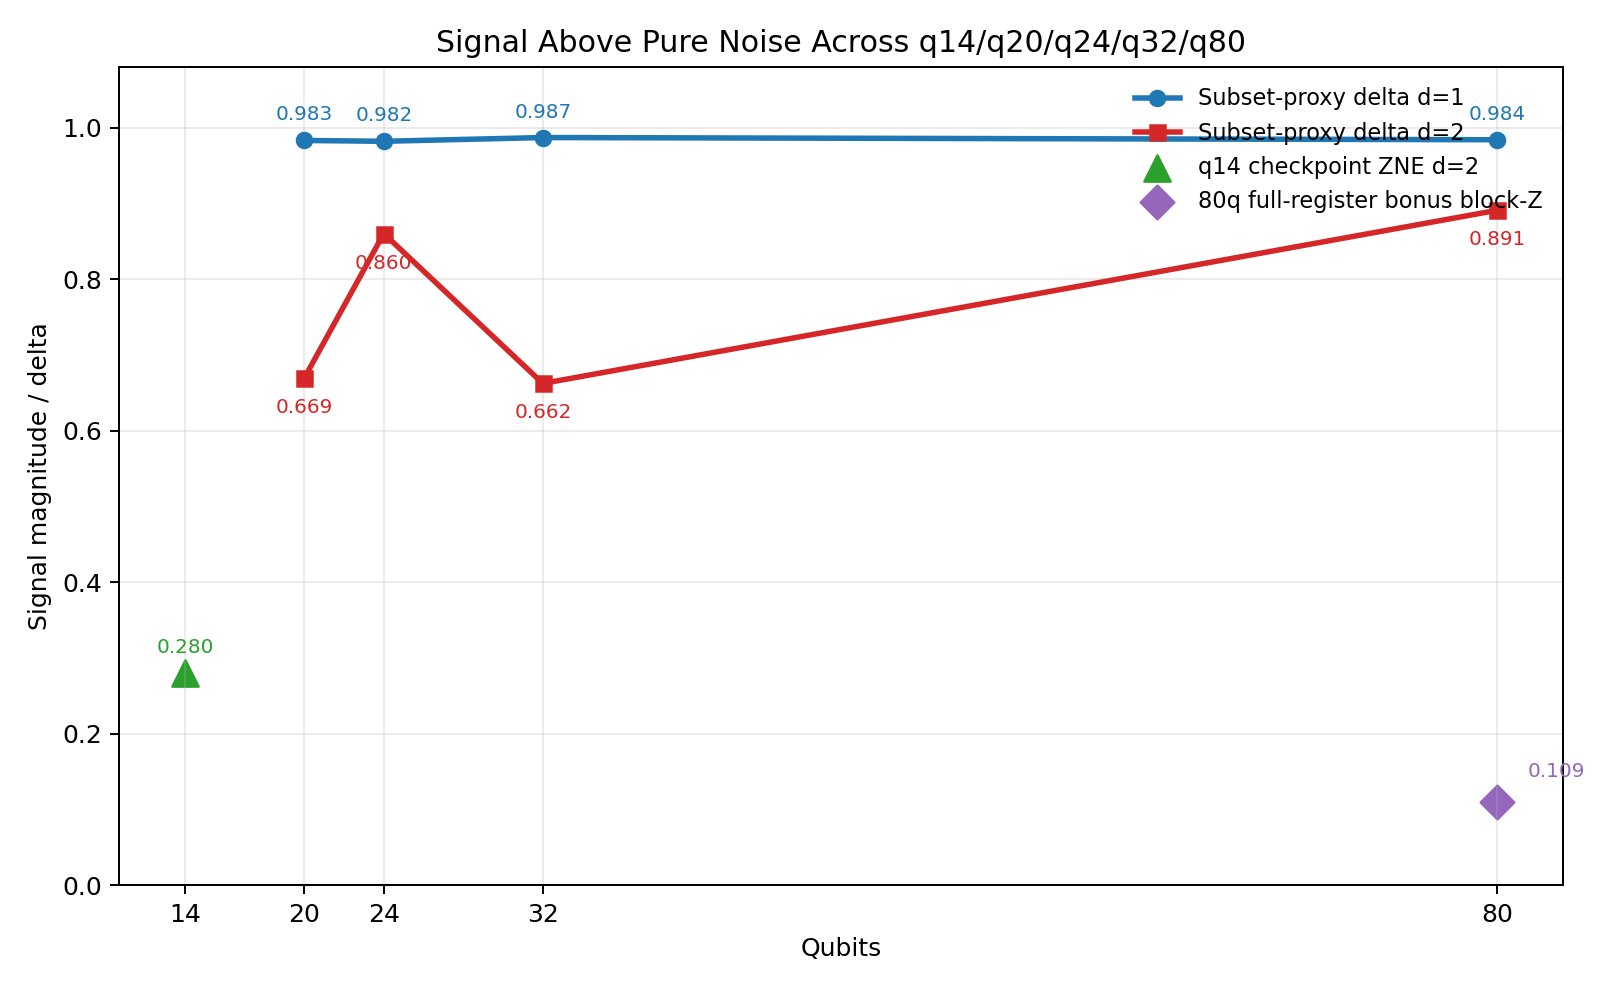
\includegraphics[width=0.96\linewidth]{figure_signal_scale.png}
\caption{Cross-scale snapshot of locality-sensitive signal magnitude across q14, q20, q24, q32, and q80. Blue and red lines show the readout-mitigated subset-proxy far-minus-overlap contrast at depths 1 and 2. The green marker shows the corrected local-fold q14 checkpoint ZNE overlap-minus-disjoint signal at depth 2, selected as the cleanest checkpoint within a broader mixed q14 hardware picture. The q80 subset point is a first \texttt{S\_A = 0..9} pilot only. The purple marker shows the exploratory 80q full-register bonus signal based on the symmetric mean absolute paired block-$Z$ linear-return delta across \texttt{front10} and \texttt{back10}. The figure should be read as a staged evidence ladder rather than as a single observable family.}
\label{fig:signal-scale}
\end{figure}

The strongest admissible q14 hardware anchor is the corrected local-fold checkpoint ZNE separation.
At depth 2, its overlap-minus-disjoint signal is 0.27957.
This is smaller than the later subset-proxy line, but still clearly positive and more disciplined than the broader whole-grid raw-versus-mitigated picture. The broader q14 readout-mitigated controls remain mixed, so this point should be read as the best admissible checkpoint rather than as uniformly positive q14 hardware behavior.

The cross-scale subset line is the main hardware result.
At depth 1, the readout-mitigated far-minus-overlap contrast remains near 0.98 for q20, q24, q32, and q80.
At depth 2, the signal decreases but remains strongly positive at every scale.
The q80 subset pilot does not collapse relative to intermediate sizes; in this snapshot it remains among the strongest shallow-depth subset contrasts. The scope remains narrower than a whole-machine statement: this is the first \texttt{S\_A = 0..9} subset pilot, not a symmetric two-subset or full-register closure.
This is the cleanest current evidence that locality-sensitive signal survives the scale-up path to 80 qubits in the subset-observable sense.

The exploratory q80 full-register bonus path is intentionally harder than the subset line.
Global full-register state-return observables proved fragile and mitigation-sensitive, so the stronger follow-up was a block-local $Z$ fallback on the same paired capture.
This gives a smaller signal, with a symmetric mirrored-block marker of 0.10932, but crucially it remains structured rather than null.
The sign pattern is spatially correct: a perturbation near $q=0$ primarily suppresses the front block, whereas a perturbation near $q=79$ primarily suppresses the back block.
The correct reading is not that the full-register route is as strong as the subset route, but that locality structure still survives after a stricter observable change.

\section{Discussion}

The black-hole motivation should enter only as an interpretation layer.
In black-hole and fast-scrambler language, the relevant physical picture is that a local perturbation rapidly spreads across many degrees of freedom so that recovery of its footprint becomes support- and time-dependent
\cite{hayden2007blackholes,sekino2008fast,maldacena2016bound}.
The present circuits are not gravity duals and do not directly test a black-hole model.
What they do test is the hardware-visible remnant of the same mechanism:
local perturbations affect nearby measured supports strongly, affect far-disjoint supports much less, and gradually erase that geometric distinction as scrambling proceeds.

That is why overlap-versus-far-disjoint controls matter.
If the observed branch separation were only a generic decay artifact, moving the perturbation site relative to the measured support would not systematically restore a large contrast.
Instead, the data show that support geometry matters strongly on the subset line and remains visible, though weaker, in the q80 block-$Z$ bonus track.

The present evidence therefore supports a two-tiered conclusion.
First, subset-level locality language is already strong through q80 on the current first-subset pilot.
Second, the stricter full-register q80 bonus track retains a smaller but nonzero structured residual signal.
What the evidence still does \emph{not} support is full-q80 OLE closure, global-q80 hardware confirmation, or a claim that the current observables already implement the final fixed-observable OLE estimator.

This is also the right place to connect to subsystem and subalgebra viewpoints.
Recent work on subsystem Loschmidt echoes and algebra-sensitive scrambling makes clear that quasi-local or restricted observables can carry scientifically meaningful scrambling information even when full-system observables are too small or too expensive to access
\cite{karch2025subsystem,andreadakis2024longtime}.
That is exactly the role played here by the q20--q80 subset line and the q80 block-$Z$ fallback.

Finally, the mitigation discussion should remain secondary to the physics claim.
The current paper benefits from local readout mitigation, M3-style comparisons, and tensor-network-inspired mitigation ideas, but the core message is not that mitigation alone created the signal.
Rather, mitigation helped reveal a signal that is already geometrically structured in the data.
For broader context on utility-scale mitigation and tensor-network error mitigation, see Refs.~\cite{filippov2023tem,filippov2024scalability}.

\section{Conclusion}

The present hardware evidence does not yet close the full fixed-observable OLE question, but it establishes a strong and useful intermediate result.
Across q20, q24, q32, and q80, shallow-depth subset-proxy locality signals remain far above a pure-noise baseline, while a stricter q80 full-register bonus analysis retains a smaller but still structured residual locality signature.
This provides a coherent staged basis for a later OLE-oriented article: the hardware signal is already there, but the final observable semantics still need to be completed explicitly.

\bibliographystyle{unsrtnat}
\bibliography{references}

\end{document}
